\documentclass[10pt]{beamer}

%%%
% PREAMBLE FOR THIS DOC 
%%%
%https://tex.stackexchange.com/questions/68821/is-it-possible-to-create-a-latex-preamble-header
\usepackage{/Users/miw267/Repos/csci246_spring2025/slides/preambles/beamer_preamble_for_CSCI246}


%%% TRY TO RESHOW TOC AT EACH SECTION START (with current section highlighted)
% Reference: https://tex.stackexchange.com/questions/280436/how-to-highlight-a-specific-section-in-beamer-toc
\newcommand\tocforsect[2]{%
  \begingroup
  \edef\safesection{\thesection}
  \setcounter{section}{#1}
  \tableofcontents[#2,currentsection]
  \setcounter{section}{\safesection}
  \endgroup
}


\usepackage[normalem]{ulem} % for strikeout (\sout)

%%%% HERES HOW TO DO IT CORRECTLY
% FIRST IN .STY FILE, DO
%\usetheme[sectionpage=none]{metropolis}
% THEN AT EACH SECTION DO
%\begin{frame}{Outline}
%  \tableofcontents[currentsection]	
%\end{frame}



%\setbeamertemplate{navigation symbols}{}
%\setbeamertemplate{footline}[frame number]{}


%%%
% DOCUMENT
%%%

\begin{document}

%\maketitle

%% Title page frame
%\begin{frame}
%    \titlepage 
%\end{frame}



\title{04/16/2025: Trees and Project Planning}
\author{CSCI 246: Discrete Structures}
\date{Textbook reference: Sec 50, Scheinerman}

\begin{frame}
    \titlepage 
\end{frame}


\begin{frame}
\small
%\begin{mygreenbox}[title=Graded Quiz Pickup]
%Quizzes are in the front of the room, grouped into four bins (A-G, H-L, M-R, S-Z) by last name. The quizzes are upside down with your last name on the back. Come find yours before, during, or after class. Only turn the quiz over if it's yours.
%\end{mygreenbox} 
%\vfill 
\begin{myredbox}[title=Announcement: Student Body Elections]
Voting is open for student body elections, which students can access on CatsConnect.
\begin{center}

\includegraphics[width=.3\textwidth]{images/voting_qr_code.png}
\end{center}
\end{myredbox}
\vfill 
\begin{myyellowbox}[title=Today's Agenda]
\begin{itemize}
	\item Reading and problems quiz (15 mins)
	\item Project overview (10 mins) 
	\item Project setup (20  mins)
\end{itemize}


\end{myyellowbox}
\vfill 

\end{frame}






\begin{frame}[standout]
Feedback on Wednesday's Quiz
\end{frame}


\begin{frame}{Reading Quiz Scores}
\small 
\begin{figure}[ht]
        \centering
        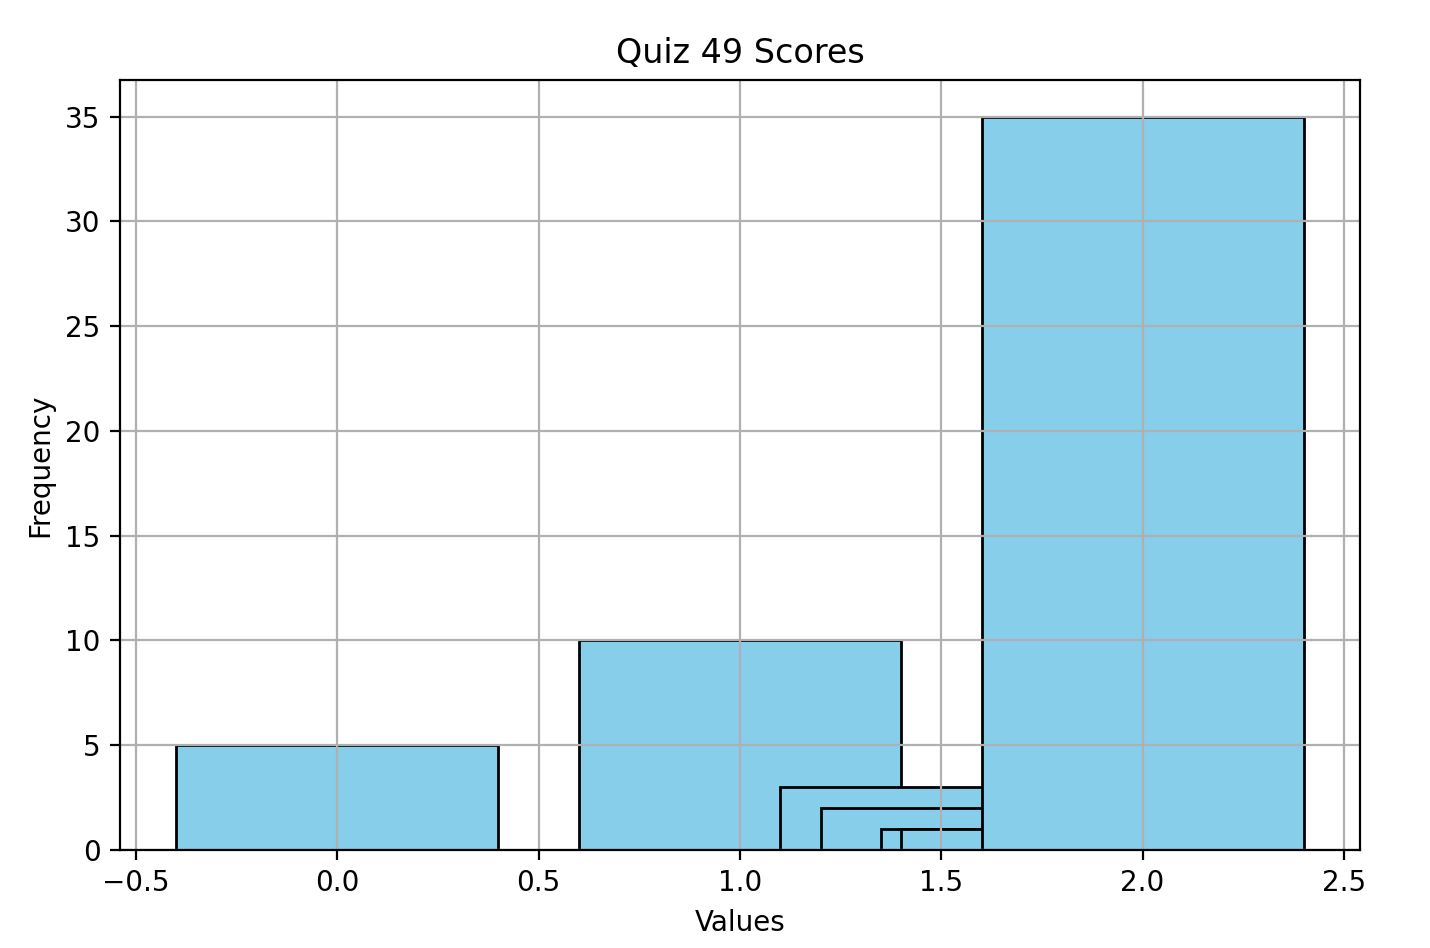
\includegraphics[width=.7\textwidth]{images/reading_quiz_scores}
   		 \caption{Median Score = 2/2 (100\%)}
\end{figure}
\vfill 
\textbf{Grading Rubric:}  
\begin{enumerate}
\item (1 point) The argument is wrong.
\item (1 point) Explanation why. (E.g. walks are not paths.)
\end{enumerate}

\end{frame}	




\begin{frame}[standout]
Today's quiz
\end{frame}

\begin{frame}
%\small 
 
\begin{myredbox}[title=\text{Reading Quiz (Trees)}]
State two different characterizations of trees. 
\end{myredbox}

\vfill
\begin{mygreenbox}[title=\text{Problems Quiz (Graph fundamentals, subgraphs, connection)}]

\begin{enumerate}
	%\item How many Hamiltonian paths does a complete graph on $n \geq 2$ vertices have? You do not need to justify this answer.
	\item How many different graphs can be formed with vertex set $V=\set{1,2,3,\hdots,n}$? Justify your answer. 
	\item (Extra credit.) Prove that in every graph, the number of vertices with odd degree is even. 
\end{enumerate}
\end{mygreenbox}
\vfill 
\begin{myyellowbox}[title=\text{Definitions (for reference)}]
Let $G$ be a graph. A path $P$ in $G$ that contains all the vertices of $G$ is called a \textbf{Hamiltonian path.}  \\
%\vspace{.1cm}

Let $G$ be a graph. If all pairs of distinct vertices are adjacent in $G$, we call $G$ a \textbf{complete graph}. 
\end{myyellowbox}
\end{frame}

\begin{frame}[standout]
\href{https://docs.google.com/document/d/1Aw7M0FXi0hPJNVsjJVT_8nUAOTVaNy-5B9RNVMiEQbs/edit?tab=t.0}{\color{blue!30}{\underline{Project Planning}}}
\end{frame}


\end{document}
